This chapter will describe three control rod decusping techniques developed as part of this work.  \hl{Say something a little more substantial}

\section{Polynomial Decusping}

The polynomial decusping technique was developed to provide a fast, simple correction to the cusping problem in the MPACT code.  This technique assumes that the reactivity and power around the partially inserted rod have a predictable shape as functions of the rod position within the MOC plane.  Based on this assumption, correction factors were developed to reduce the volume fraction of control rod material and reduce the magnitude of the cusping effects.

To do this, a 3$\times$3 assembly problem with a control rod in the center assembly was used (this problem is described in more detail in Section \hl{number}).  

\section{Subplane Collision Probabilities}

The subplane scheme as it was originally conceived was used primarily to address stability issues caused by thin MOC planes in early 2D/1D codes.  While other improvements to the 2D/1D method have largely eliminated these problems, the idea of capturing subplane information using the subplane scheme can be useful for addressing partially inserted rods without substantially increasing the computational cost.  To do this, three changes were made to the basic subplane scheme: an axial correction, a radial correction, and an MOC cross section correction.

\subsection{Axial Correction}

Traditionally, the subplane scheme uses axially constant cross sections for all subplanes in each MOC plane.  When a control rod is partially inserted in the plane, a flux-volume homogenized cross section is calculated and used for each subplane.  This allows the subplane scheme to be used, but does little to account for the partially inserted rod.

To resolve this issue, the subplanes with the control rod use the rod cross section, and the subplane without the rod use the moderator cross section.  These cross sections are still homogenized using flux-volume weighting as before, but without homogenizing axially.  Doing this allows both the CMFD and P$_3$ calculations to capture some of axial effects of the partially inserted rod, reducing the magnitude of the cusping errors around the rod.

\subsection{Radial Correction}

Using axially heterogeneous cross sections within an MOC plane corrects some of the cusping effects, but it does not accurately capture the radial effects of the partially inserted rod.  In reality, the radial flux shape in the rodded subplanes is completely different from the shape in the unrodded subplanes.  The MOC calculations are done on the thicker MOC planes using axially homogenized cross sections in the partially rodded regions.  This produces a radial flux shape that is not representative of either the rodded or unrodded region, as illustrated in figure \hl{number}.  Thus, using this radial flux shape to calculate the pin-homogenized cross sections for CMFD P$_3$ introduces some error in the cross sections.

\begin{figure}
    \centering
    \caption{Radial flux shapes for rodded, unrodded, and axially homogenized MOC pin cells}\label{f:radialFluxProfiles}
\end{figure}

To account for this, a 1D collision probabilities calculation is introduced during the homogenization step.  These calculations are done in the rodded and unrodded regions to generate separate radial flux shapes that can be used during the CMFD homogenization step, as shown in Figure \ref{f:SCPdecusping}.  These CP calculations are done for each energy group and consist of inverting a small $N_r \times N_r$ matrix, where $N_r$ is the number of rings in the pin cell model (usually less than 10).  Because these matrices are so small, these calculations are computationally negligible when compared with the full 2D/1D iteration scheme while providing more accurate radial information for the cross section homogenization.

\begin{figure}
    \centering
    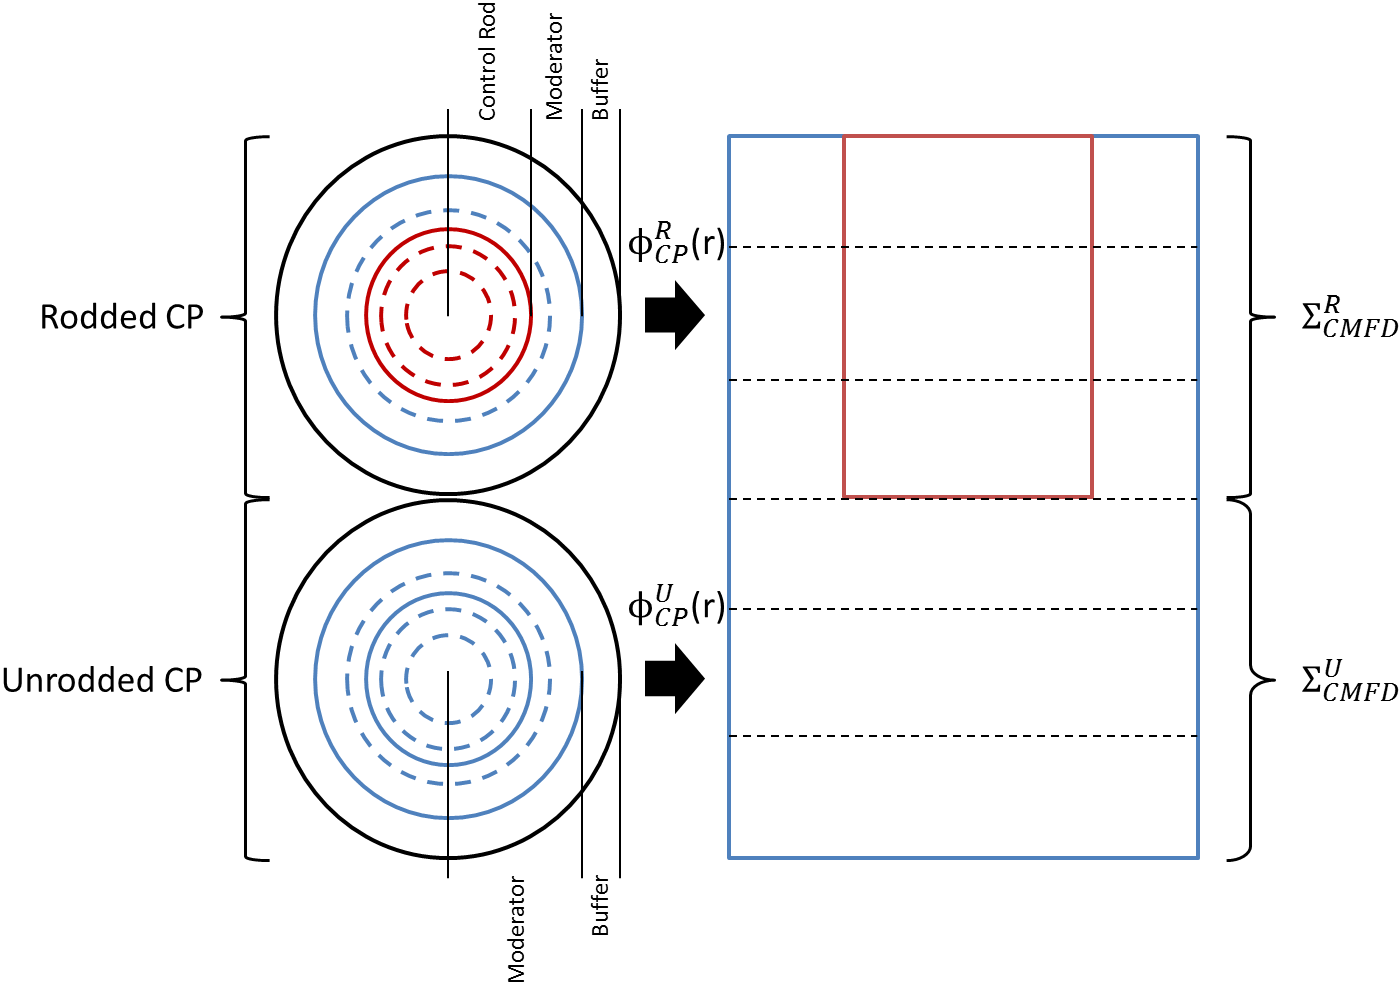
\includegraphics[width=0.8\textwidth]{CPdecusp.png}
    \caption{Illustration of subplane collision probabilities used on a partially inserted rod}\label{f:SCPdecusping}
\end{figure}

\subsection{MOC Correction}

The final step in this decusping technique is to use the subplane information from the CMFD/P$_3$ calculations to improve the MOC calculations.  To do this, the volume-homogenized cross sections are updated each iteration using a flux-volume weighting that involves the axial flux shape from the CMFD/P$_3$ system and the radial flux shape from the CP calculations.  These are combined the same was as the nTRACER method using Equation \ref{e:nTRACERdecusping}.

\section{Subray Method of Characteristics}

\begin{figure}
    \centering
    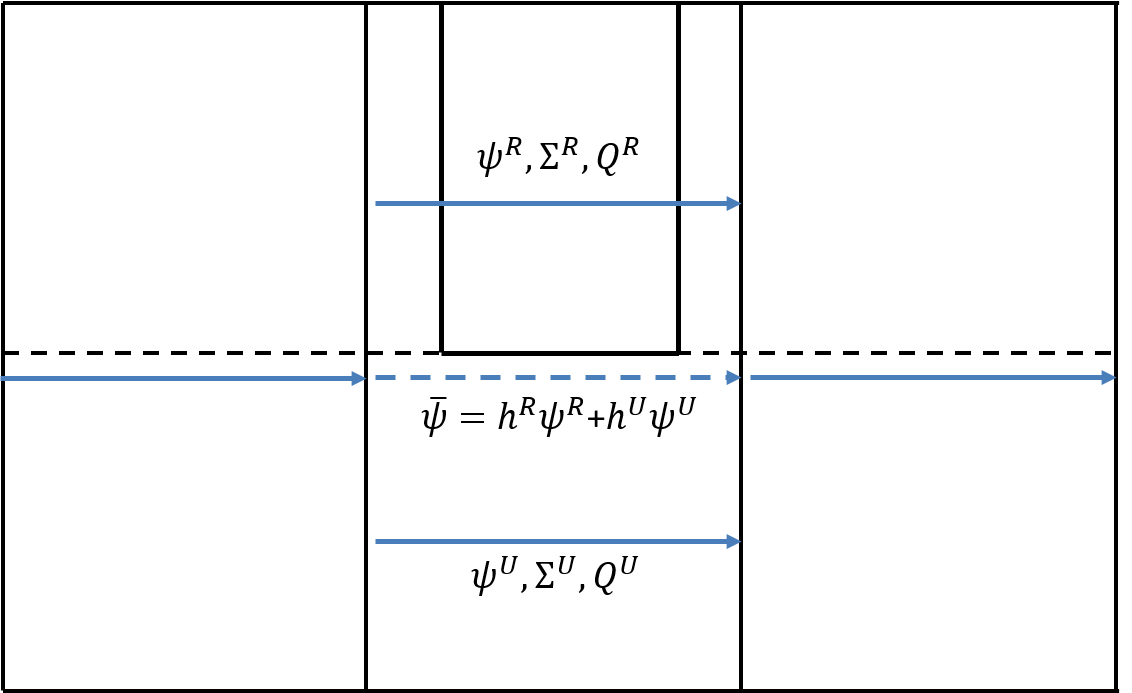
\includegraphics[width=0.8\textwidth]{sub-ray_illustration.png}
    \caption{Illustration of subray method of characteristics for partially inserted rod}\label{f:subrayMOC}
\end{figure}